\documentclass{beamer}
\usepackage[utf8]{inputenc}
\usepackage[MeX]{polski}
\usepackage{graphicx}
\usepackage{listings}
\usepackage{array}
\usepackage{xcolor}
\usepackage{colortbl}
\usepackage{subfig}
\usetheme{Warsaw}
\usecolortheme[rgb={0,0.5,1}]{structure}
\setbeamerfont{title}{family=\rm}
\setbeamerfont{author}{family=\it}
\title{Bezpieczeństwo danych na dysku\\ w świecie internetu}
\subtitle{SCR - Systemy Operacyjne}
\author{Michał Wieczorek}
\institute{
Automatyka i Robotyka,
Wydział Elektroniki\\
Politechnika Wrocławska}

\begin{document}
\begin{frame}
\titlepage
\end{frame}

\section{Spis treści}
\begin{frame}
	\frametitle{Plan prezentacji}
	\tableofcontents
\end{frame}

\section{Struktura systemu}
\begin{frame}
	\frametitle{Struktura systemu}
	\begin{figure}[H]
	\centering
	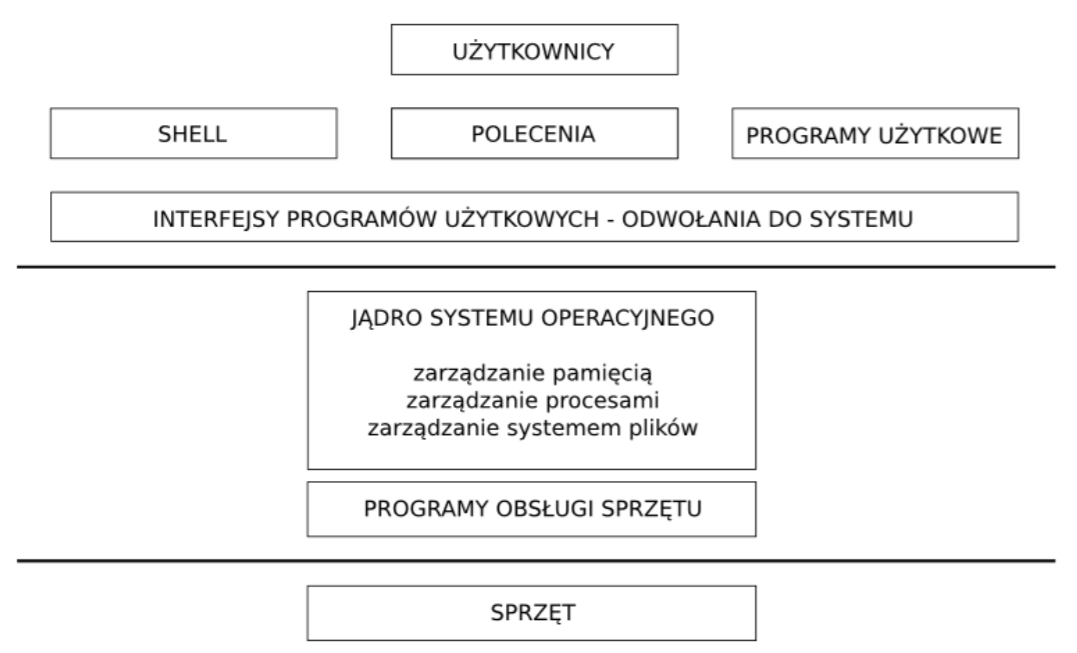
\includegraphics[width=1\textwidth]{podzial.png}
	\end{figure}
\end{frame}

\section{Rodzaje zagrożeń}
\subsection{Buffer Overflow}
\begin{frame}
	\frametitle{Rodzaje zagrożeń}
	\begin{figure}[H]
	\centering
	
\includegraphics[width=0.8\textwidth]{overflow2.png}
	\end{figure}
\end{frame}

\subsection{Exploit}
\begin{frame}
	\frametitle{Rodzaje zagrożeń}
	\begin{figure}[H]
	\centering
	
\includegraphics[width=1\textwidth]{exploit.png}
	\end{figure}
\end{frame}

\subsection{Kernel drivers}
\begin{frame}
	\frametitle{Rodzaje zagrożeń}
	\begin{figure}[H]
	\centering
	
\includegraphics[width=0.5\textwidth]{drivers.png}
	\end{figure}
\end{frame}

\subsection{Statystyka}
\begin{frame}
	\frametitle{Rodzaje zagrożeń}
	\begin{figure}[H]
	\centering
	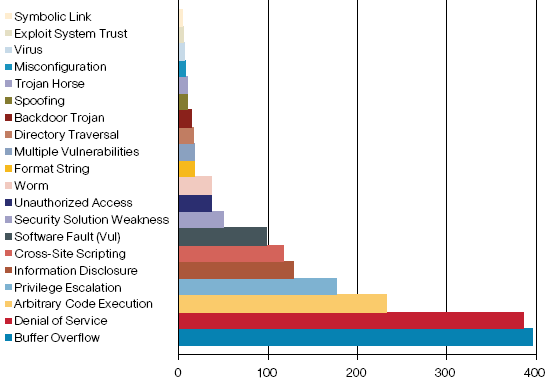
\includegraphics[width=0.9\textwidth]{overflow.png}
	\end{figure}
\end{frame}

\section{Metody zabezpieczania}
\begin{frame}
	\frametitle{Podział zabezpieczeń na 3 główne grupy}	
	\begin{itemize}
	\item Mechanizmy filtrowania ruchu sieciowego
	\item Wykrywanie włamań i kontrola plików
	\item Ograniczenie szkód wywołanych włamaniem
	\end{itemize}
\end{frame}

\subsection{Filtrowanie ruchu sieciowego}
	\begin{frame}
	\frametitle{Filtrowanie ruchu sieciowego}
	\begin{figure}[H]
	\centering
	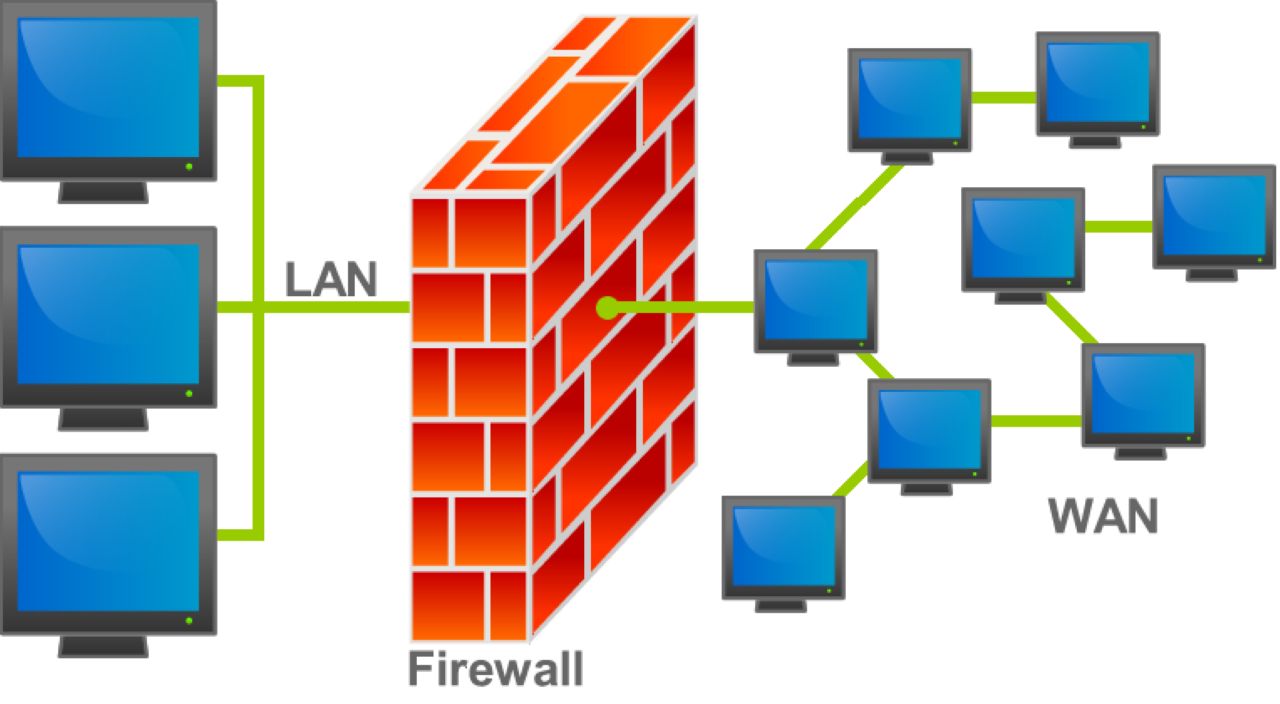
\includegraphics[width=1\textwidth]{firewall.png}
	\end{figure}
\end{frame}

\subsection{Wykrywanie włamań i kontrola plików}
\begin{frame}
	\frametitle{Wykrywanie włamań i kontrola plików}
	\begin{figure}[H]
	\centering
	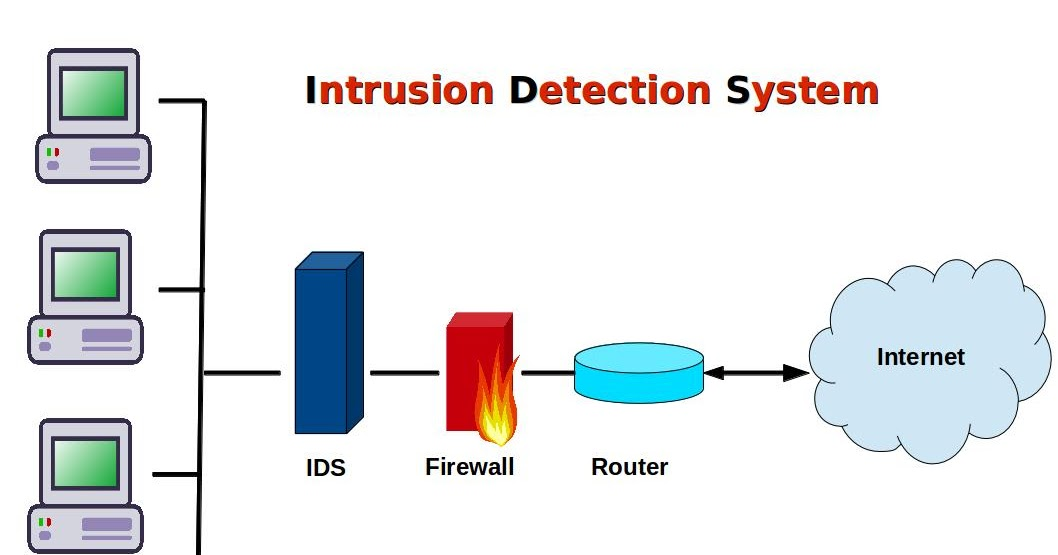
\includegraphics[width=1\textwidth]{ids.png}
	\end{figure}
\end{frame}

\subsection{Ograniczenie szkód wywołanych włamaniem}
\begin{frame}
	\frametitle{Ograniczenie szkód wywołanych włamaniem}
	\begin{figure}[H]
	\centering
	
\includegraphics[width=1\textwidth]{selinux.png}
	\end{figure}
\end{frame}

\begin{frame}
	\centering
	\frametitle{Zakończenie}
	Dziękuję za uwagę :)
	\end{frame}
\end{document}